\section{Seasonal Reckoning using Daily Eclipses}
\emph{Chronological ID:} \texttt{2024-01-28:01}

\emph{Structural ID:} \texttt{2.2.1.2}

\begin{figure}[h]
  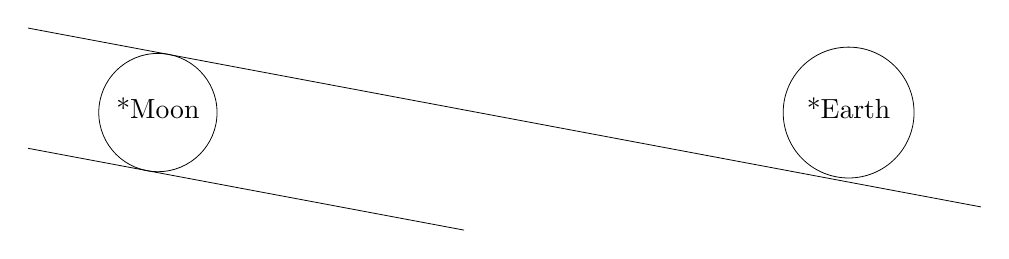
\begin{tikzpicture}
    \draw[black,line width=0.01cm] (1.649, 1.493) circle (0.751cm);
    \draw[black,line width=0.01cm] (10.421, 1.493) circle (0.831cm);
    \draw[black,line width=0.01cm] (0.0, 2.566) -- (12.1, 0.295);
    \draw[black,line width=0.01cm] (0.0, 1.039) -- (5.537, 0.0);
    \node[anchor=south] (lm) at (1.649, 1.293){*Moon};
    \node[anchor=south] (le) at (10.421, 1.293){*Earth};
  \end{tikzpicture}
  \caption{Illustration of eclipse geometry during a solstice.}
\end{figure}

Due to an axial tilt of the *Moon, the *Earth and their orbit around each other of 10.63$\degree$ relative to the ecliptic, ``traditional'' seasonal variation, that is, the variation in weather due to certain regions being tilted towards or away from the *Sun, is less noticeable than it would be if the axial tilt was closer to Earthly levels. However, in lieu of this, a different seasonal effect presents itself: regular solar eclipses.

On the near side of the *Earth, no region avoids solar eclipses entirely. However, their seasonality differs: equatorial regions experience solar eclipses, every day, for a period of time centered on the equinoxes, while polar regions experience them for two periods of time symmetrically positioned with the winter solstice acting as the axis of symmetry. This results in rather long periods of darkness and low temperatures in the polar regions, which results in consistent wind away from the equator, subject to the Coriolis effect.

Interestingly, on the equator on the near side, the ``seasons'' repeat twice a year, rather than once a year.

In addition to solstices and equinoxes, local calendar makers have found another time of year useful to insert into the calendar: whenever the eclipse shadow starts/stops intersecting the equator. There are 4 such moments in a year.

Lunar eclipses, visible from all of the *Earth's near side, are also useful for the need to accurately determine a calendar.
\newpage
